\section{Methodology}
This section will mainly cover the basic statistical properties which needs to be addressed in order to handle time series data, as well as the theories behind the models utilized for predictions. Going over the features of data used in this paper in subsection 2.1, 2.2 the features of the dataset and the pre-processing of data which remedies some of the problematic statistical properties would be mentioned. In subsection 2.3 and 2.4, the modelling process behind the conventional model and the deep learning model will be discussed respectively. 

\subsection{Dataset}
This paper uses three datasets which are released from the government. 2 datasets are from the Tokyo Bureau of Social Welfare and Public Health which contains information about the daily observed COVID-19 numbers, hospital vacancy, and PCR results conducted in Tokyo prefecture. The other dataset is from the Cabinet Secretariat of Japan which releases daily numbers of foot traffic data observed in Shinjuku Station. All of the datasets used in this paper are captured in daily spans and the range of the data is fixed from May 2nd, 2020 to December 30th, 2021 for all features \citep{tokyo_COVID,tokyo_pcr, tokyo_foot_traffic}.  In this paper, we will concatenate all 3 datasets into 1 master dataset and construct our models.\\ 

\begin{figure}[!ht]
    \centering
    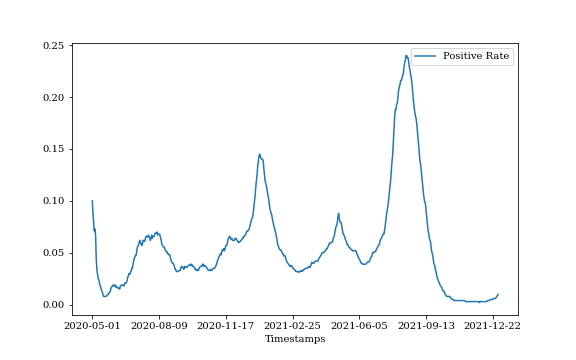
\includegraphics[width=12cm]{images/Positive_Rate.png}
    \caption{This shows an example of a time series line plot. The blue line represents the value of data point at a given timestamp. }
    \label{fig:lline_positive}
\end{figure}
The total number of time steps captured in this dataset is \textbf{608 rows} by \textbf{12 columns}.

\noindent The features are as follows:
\begin{itemize}
\item \textbf{Date}: The daily timestamps
\item \textbf{Hospitalized}: The number of patients being hospitalized on that date
\item \textbf{Light-Mid\_Symptoms}: The number of patients who have light-mid symptoms on that date
\item \textbf{Severe\_Symptoms}:  The number of patients who have severe symptoms on that date 
\item \textbf{Dead}: Daily Death tolls
\item \textbf{Discharged}: The number of patients who are discharged from hospitals on that date 
\item \textbf{PCR\_Positive}: The number of people who are tested positive in PCR testing on that date
\item \textbf{PCR\_Negative}: The number of people who are tested negative in PCR testing on that date
\item \textbf{Tested\_MA(7days)}: The moving average of the number of PCR tests done within the last 7days
\item \textbf{ComparisonPreDay}: The percent change of the population growth rate compared to the former day
\item \textbf{ComparisonPreDeclare}: The percent change of the population growth rate compared to the population during the 3rd Emergency Declaration issued in January 7th, 2021
\item \textbf{ComparisonPreSpread}: The percent change of the population growth rate compared to the average population during pre-COVID-19 span (January 18th, 2020 - February 14th, 2020)
\end{itemize}

\subsection{Dataset Pre-processing}
\subsubsection{Standardization}
The aforementioned features vary in terms of numerical characteristics from decimals to percentage points. In this paper, all the features within the dataset is standardized from its individual mean and standard deviation defined as:

\begin{equation}\label{eq:standardized}
    X_{\mathrm{std}} =\frac{X - \mu}{\sigma} ,
\end{equation}
where $X$ are the input data, $\mu$ is the mean of the featured data, $\sigma$ is the standard deviation of the featured data, and $X_\mathrm{{std}}$ is the standardized data. 

Added to the pre-processing of individual data, there are several statistical properties that each time series data needs to fulfill in order to induce an accurate prediction. Below would explain several statistical features the data needs to fulfill. 

\subsubsection{Stationarity}
Stationarity in time-series data is when the statistical properties, such as the mean, variance, and the covariances between given time periods are constant over time. Assuring stationarity within the dataset precludes the risk of having a spurious forecast result \citep{granger_spurious_1974}.

\begin{figure}[!ht]
    \centering
    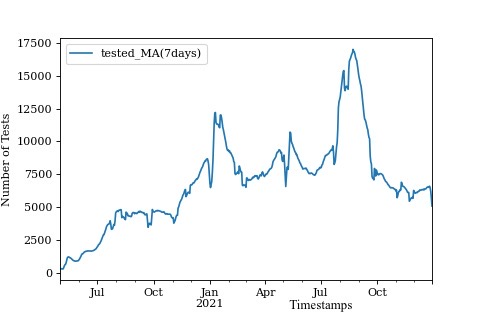
\includegraphics[width=10cm]{images/Non_stationary.png}
    \caption{The feature \textbf{tested\_MA(7days)} has an upward incline and the mean at a given time is not constant throughout the timestamps. This statistical feature represents a non-stationary process.}
    \label{fig:non-stationary}
\end{figure}

In Figure \ref{fig:non-stationary}, we see that there is a positive trend in our values as time progress. This violates the condition of having a fixed mean over time, hence we could conclude that this process is non-stationary. 

To numerically determine if the dataset is in fact stationary or non-stationary, we conduct a unit root test, checking the presence of a unit root within the time series data. There exists many unit root tests, but this paper would focus on the Augmented-Dickey Fuller (ADF) test \citep{ADF}. Below would be a brief summary cited from the works of \citet{ADF, ADF_test_statistic}. For explanation of ADF test, we assume an observed time series data of $Y_{1}, Y_{2},\ldots, Y_{N}$ and a differential-form autoregressive equation $\Delta Y_{t}$ as:

\begin{equation}\label{eq:AR}
    \Delta Y_{t}=\alpha+\boldsymbol{\beta} t+\gamma Y_{t-1}+\sum_{j=1}^{p-1}\left(\delta_{\mathrm{j}} \Delta Y_{t-j}\right)+\varepsilon_{t} ,
\end{equation}
where $\Delta$ is the first difference operator, $t$ is the time index, $\alpha$ is the intercept constant often called as drift, $\beta$ is the coefficient of a time trend, $p$ is the maximum lag order of the autoregressive process, and $\varepsilon$ is an independent identically distributes residual term.

The specifications varies different depending on the deterministic elements presented in the time series data; if there is a drift in the data $\alpha\neq0$, if there is also a linear trend $\beta\neq0$, and if neither drift nor linear trends and are present, we illustrate by $\alpha = 0, \beta = 0$. We do a hypothesis test if the coefficient $\gamma$ is equal to $0$, which means that the autoregressive process possesses a unit root. Hence, the null hypothesis and the alternative hypothesis is defined as:

\begin{align}\label{eq:ADF_hypothesis}
    H_{0}&: \gamma = 0 \mbox{ (unit root exist and hence non-stationary)}.\\
    H_{1}&: \gamma < 0 \mbox{ (no unit root and hence stationary)}.
\end{align}
The test statistic is defined as:

\begin{equation}\label{eq:ADFt}
    ADF_{\mathrm{t}}=\frac{\hat{\gamma}-1}{\operatorname{SE}(\gamma)} , 
\end{equation}
where $\hat{\gamma}$ is the least squares estimate. To test the null hypothesis, we compare this test statistic with the critical value and rejects the null hypothesis when the test statistic is less than the critical value. In this paper, the ADF test is implemented using the \textsc{adfuller} module provided by the \textsc{statsmodels} library \citep{statsmodels_ADF}. 

\subsubsection{First Differencing}
When the time series is found to be a non-stationary process, there is a need to convert our process into a stationary process. In this paper, a method called first differencing is applied to remedy the non-stationary process. For a given time series $Y_{t}$, the procedure of first difference is defined as:
\begin{equation}\label{eq:First_Difference}
    \Delta Y_{\mathrm{t}} = Y_{\mathrm{t}} - Y_{\mathrm{t-1}},
\end{equation}
where $t$ is the given time period and $\Delta$ is the first difference operator. 

\begin{figure}[!ht]
    \centering
    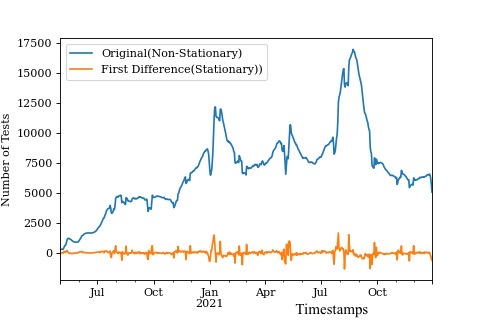
\includegraphics[width=10cm]{images/First_Difference.png}
    \caption{The blue line represents the original time series of \textbf{Tested\_MA(7days)}. The orange line represents the same data feature but after the First Difference is taken. We could see that the modified time series converges close to the axis of 0 and the mean is constant throughout time. Hence, we could now visually indicate that the process has become stationary.}
    \label{fig:First difference}
\end{figure}

As apparent from Figure \ref{fig:First difference} we could indicate a positive trend in our original data of feature \textit{Tested\_MA(7days)}. This indicates that the original data does not fulfill the condition of stationarity from the attribute that the mean alters within different given time. By applying the first difference, the data is now converged close to the axis and do not indicate any drift, hence stationary. Therefore, applying the first difference for the features which is non-stationary in our data establishes a robust foundation for our predictive model. 

\subsubsection{Multicollinearity}
Multicollinearity refers to the linear relationship between two or more time series data. More specifically, there is multicollinearity when there is high correlation among 2 or more independent variables. Figure \ref{fig:multicollinearity} shows the multicollinearity of the \textit{Hospitalized} feature and \textit{Light-Mid\_Symptom} feature in our data. We could see that the lines are identical and the quantile-quantile plot is linear. Multicollinearity presents detrimental issues in the precision of regression models, whereas the statistical significance of independent variables are undermined due to the partial regression coefficient becoming highly volatile between different samples \citep{multicollinearity_problem}.

\begin{figure}[!ht]
    \centering
    \subfloat[\centering Line graph of \textbf{Hospitalized}(blue) and \textbf{Light-Mid\_Symptoms}(orange). ]{{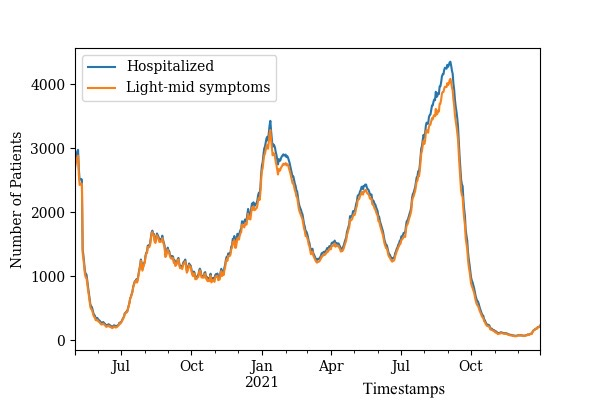
\includegraphics[width=6.3cm]{images/Multicollinearity.png} }}%
    \qquad
    \subfloat[\centering Quantile-Quantile plot of \textbf{Hospitalized} and \textbf{Light-Mid\_Symptoms} ]{{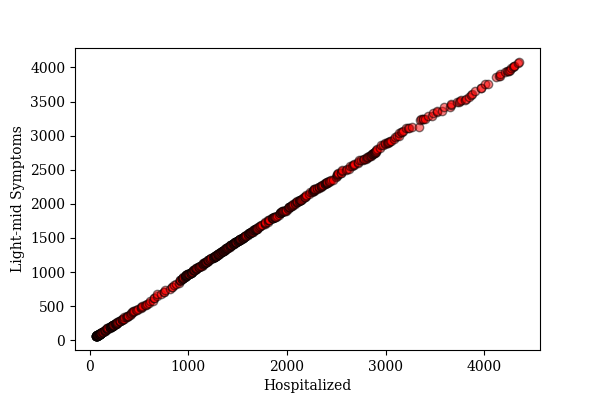
\includegraphics[width=6.3cm]{images/QQplot_multicollinearity.png} }}%
    \caption{Figure (a) shows a line plot of two datasets. By plotting them together, the lines indicate an identical trend and is in complete align with each other. From this property, we can indicate multicollinearity within these two data features. Figure (b) is the Q-Q plot for the same datasets. Q-Q plots show whether two given datasets have a similar probability distribution. Using the Q-Q plot we can visually see that the plot of the given dataset is in complete linear relation, which indicates that these two features have a very identical distribution over its respective datasets.}
    \label{fig:multicollinearity}
\end{figure}

To detect multicollinearity within the dataset, the Variance Inflation Factor (VIF) is popularly used defined as:

\begin{equation}\label{eq:VIF}
    VIF_{i}=\frac{1}{1-R_{i}^{2}} ,
\end{equation}
where $R_{i}$ is the Coefficient of determination for the $i$th individual variable. A large value in $VIF$ indicates high linear dependency in its variables and the threshold to determine from high to low is generally set at 10 \citep{multicollinearity_VIF}. In this paper, the diagnosing of multicollinearity is implemented using the \textsc{variance\_inflation\_factor} module provided by the \textsc{statsmodels} library \citep{statsmodels_VIF}.
Despite multicollinearity causing detrimental effects to the precision of regression models, there are no concrete methods to remedy the statistical feature altogether. In this paper, the explanatory variables which presented high VIF are excluded from the model to avoid jeopardizing the accuracy of predictions. 

\subsection{Conventional Models}
In this paper, several conventional models are used as baseline models to compare the precision of the predictions with the deep learning models. 
\subsubsection{ARMA model}
The \textit{Autoregressive Moving Average (ARMA)} model is a univariate time series model which is widely used for forecasting values. \textit{ARMA} integrates features of \textit{Autoregressive(AR)} model and \textit{Moving Average(MA)} model. When assuming a non-stationary process in the objective model, Autoregressive Integrrated Moving Average (ARIMA) model is used, which takes the differencing process (defined in equation \ref{eq:First_Difference}), into account to convert the process into a stationary time series. In our paper, a preprocessed dataset which already passes the ADF test prior to the modelling process will be used in the modelling process, hence \textit{ARMA} model will be discussed.

AR model assumes that the objective values depend on the values from the past, hence can seek a regressive relationship between past values and future values. MA model on the other hand, focuses on the error term in which the linear regression was unable to incorporate. Finally, by incorporating features of the regressive relationship in the AR model, and the patterns in the error term captured by the MA model we get the ARMA model which is capable to illustrate more complex time series. The AR model, MA model, and ARMA model are defined as:

\begin{align}\label{eq:ARMA}    
    \mathrm{A R}(p)&: Y_{t}=c+\sum_{i=1}^{p} \phi_{i} Y_{t-i}+\epsilon_{t},\\
    \mathrm{M A}(q)&: Y_{t}=c+\sum_{i=1}^{q} \theta_{i} \epsilon_{t-i}+\epsilon_{t},\\
    \mathrm{A R M A}(p, q)&: Y_{t}=c+\sum_{i=1}^{p} \phi_{i} Y_{t-i}+\sum_{i=1}^{q} \theta_{i} \epsilon_{t-i}+\epsilon_{t},
\end{align}
where $Y$ is the objective value, $t$ is the given time period, $c$ is the constant accounting for the drift, $p$ and $q$ are the amount of lags used to regress with the value of prediction, $\phi$ and $\theta$ are the corresponding coefficient of the past objective values, and past error terms respectively, and $\epsilon$ is the error term. Conventionally, the lag terms in each of these models will be written in parenthesis after the model name such as $\mathrm{A R M A}(p, q)$ in  (\ref{eq:ARMA}). 

In this paper, the ARIMA model will be used as a baseline model for the univariate prediction section. Therefore, if the prediction error in this model is bigger than the neural network model, it suffices to say that the deep learning is ineffective in its prediction. 

\subsubsection{VARMA model}
The \textbf{Vector Autoregressive Moving Average (VARMA)} model is a mutivariate time series model which converts the coefficient of ARMA model into a finite vector space corresponding to the number of features included in the model. Therefore, the characteristic of the model incorporating more information within the model is advantageous if the data of our objective value is generated from a complex latent structure. 

Below would be a brief summary by \citet{VARMA} about the essential theories of VARMA model. Assuming multiple $K$-dimensional stationary time series $y_{1}\ldots y_{T}$, the VARMA model can be expressed in the general form of:

\begin{gather}
\begin{array}{l}\label{eq:VARMA_general}
    A_{0} y_{t}=A_{1} y_{t-1}+\cdots+A_{p} y_{t-p}+M_{0} u_{t}+M_{1} u_{t-1}+\cdots+M_{q} u_{t-q}, \\
    \quad t=0, \pm 1, \pm 2, \ldots,
\end{array}
\end{gather}
where $A_{0}, A_{1}, \ldots, A_{p}$ are $(K \times K)$ matrices which stores autoregressive coefficients and $M_{0}, M_{1}, \ldots, M_{q}$ also being a $(K \times K)$ matrices which stores moving average coefficients. 

\noindent By defining the VAR and MA operators respectively, as $A(L)=A_{0}-A_{1} L-\cdots-A_{p} L^{p}$ and $M(L)=M_{0}+M_{1} L+\cdots+M_{q} L^{q}$, where $L$ is the \textit{backshift operator},  (\ref{eq:VARMA_general}) can be written in more compact notation as:

\begin{equation}\label{VARMA_abbr}
    A(L) y_{t}=M(L) u_{t}, \quad t \in \mathbb{Z},
\end{equation}
where $u_{t}$ is a white-noise process. 

In this paper, VARMA model will be used as a baseline model of the multivariate time series prediction and will be compared with the performance of neural network models. Therefore, if the prediction error in the VARMA model is smaller than the neural network models, it will be concluded that deep learning methods do not suggest a sufficient replacement with the conventional time series forecasting methods. 

\subsubsection{Model Selection Process}
In both \textbf{ARMA} and \textbf{VARMA} models, we set the order $p, q$ for the autoregressive model and moving average model, respectively. The values are set to determine the amount of past values the model will use to determine future values. There are various ways to determine the amount of order, but this paper will be concerned with two model selection criteria; Akaike Information Criterion (AIC) and Bayesian Information Criterion (BIC). Below will be a brief summary of both AIC and BIC using the works of \citet{AIC_BIC} for reference. 

AIC was developed by \citet{AIC} to provide an adequate hypothesis testing procedure to identify the optimal statistical model. Let us assume a candidate model $M_{k}$ with dimension $k$. The AIC is defined as:

\begin{equation}\label{eq:AIC}
    \mathrm{AIC}=-2 \ln L\left(M_{k}\right)+2 k,
\end{equation}
where $L(M_{k})$ is the likelihood corresponding to the model $M_{k}$. Looking at the first term $-2 \ln L(M_{k})$, we could see that this term is the residual sum of squares corresponding to the model for the linear regression model with a Gaussian likelihood which can be shown as:
\begin{equation}\label{eq:AIC_first_term}
    -2 \ln L\left(M_{k}\right)=\sum_{i=1}^{n}\left(y_{i}-x_{i}^{\top} \widehat{\beta}\left(M_{k}\right)\right)^{2},
\end{equation}
 where $\widehat{\beta}\left(M_{k}\right)$ is the least squares estimator for model $M_{k}$. This indicates that the first term of (\ref{eq:AIC}) is the amount of loss of the model $M_{k}$ with the true observed value, which is preferred to be minimized. The AIC also penalizes the model of having large dimensions by adding the second term of (\ref{eq:AIC}). 

\noindent Therefore, the model which minimizes the value of AIC will be considered to be the best model, and we apply this to evaluate the optimal lag length of the considered model. 

An alternative information criteria used for model selection is called the BIC. Developed by \citet{BIC}, the BIC has modified the maximum likelihood estimators in the works of \citet{AIC}. Let us assume again a candidate model $M_{k}$ with dimension $k$. The BIC for this model is defined as:
\begin{equation}\label{eq:BIC}
    \mathrm{BIC}\left(M_{k}\right)=-2 \ln L\left(M_{k}\right)+\ln (n) k,
\end{equation}

\noindent where $n$ is the sample size. Similar to AIC, the model which minimizes the value BIC will be considered the optimal model within the candidate model. Compared to AIC, the penalty term in BIC, which is represented as $\ln (n) k$, is much harsher. Therefore, when using BIC we get a sparser model compared to AIC. 

In this paper, these information criterion will be used to determine the lag length of our conventional models. 

\subsection{Deep Learning Models}
With the expanding availability of huge datasets and high speed computing technology becoming more affordable, Deep learning modelling is becoming a popular method of predicting future value for its high accuracy. Deep Learning methods is accustomed to solve two major domains of issue which are classification and regression. In this paper, we will use multivariate data to predict the value of one objective value, which can be classified as regression problem. Below would go over the theories and basic structure of the models used in this paper.
\subsubsection{Deep Neural Networks for Regression Problem}
\begin{figure}[ht]
    \centering
    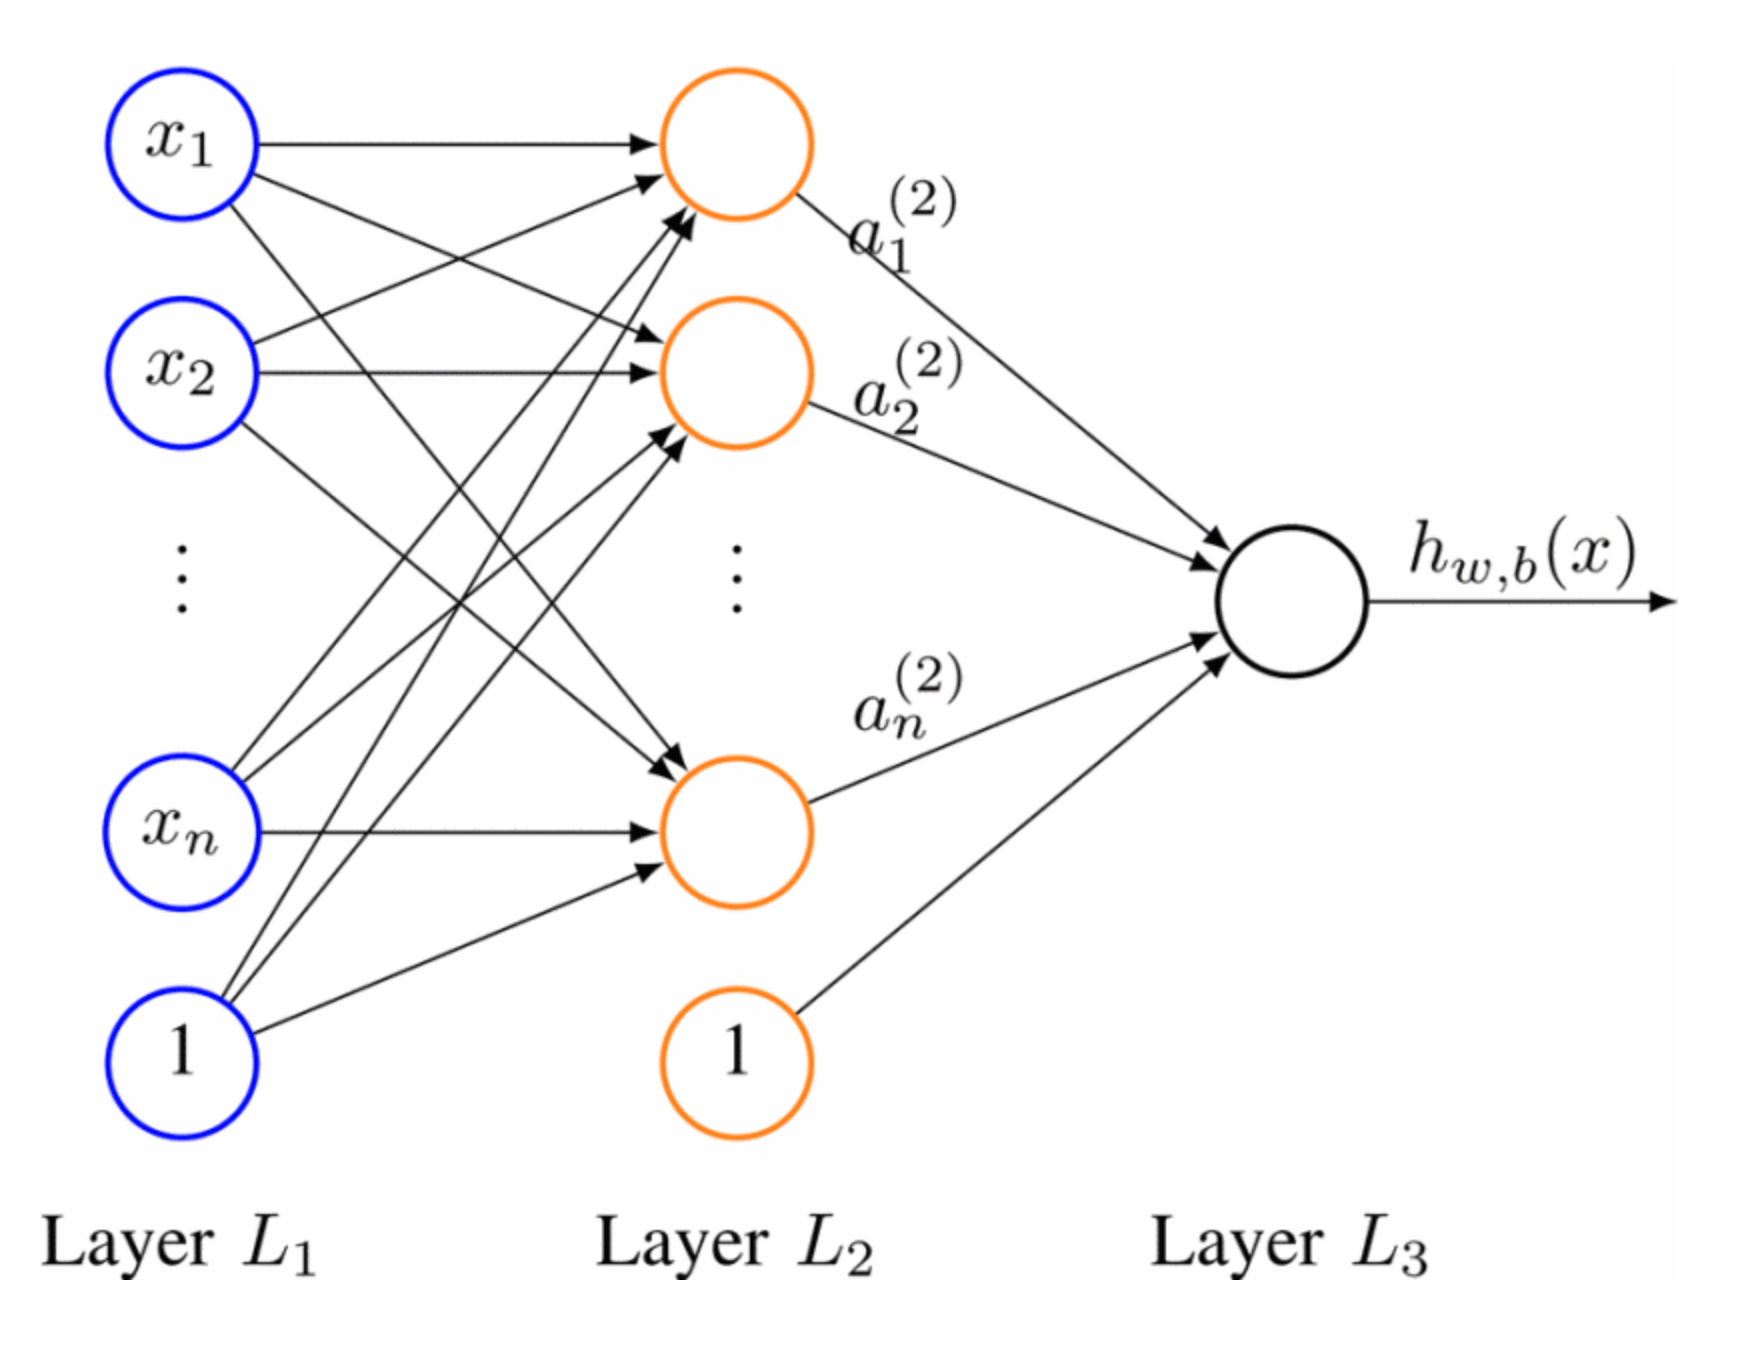
\includegraphics[width=12cm]{images/Neural_Network.png}
    \caption{Basic Structure of Neural Network\citep{NNStructure}. The layers indicate a chain of nodes and each nodes are connected with all the nodes in the next layer. }
    \label{fig:Neural_Network}
\end{figure}
Neural Network refers to the structure in which chains of perceptron being connected in multiple layers. We see from Figure \ref{fig:Neural_Network} that the neural network consists of multiple layers and each perceptrons inside the layers are connected with all the perceptrons inside the next layer. The first layer (Layer $L_{1}$ in figure \ref{fig:Neural_Network}) is called the \textit{input layer} which act as a gate for all input data. The last layer (Layer $L_{3}$ in figure \ref{fig:Neural_Network}) is called the \textit{output layer} which stores the final outcome of the data which went through the defined network. The layers between \textit{input layer} and \textit{output layer} is called the \textit{hidden layer(s)} (Layer $L_{2}$ in figure \ref{fig:Neural_Network}) which receives the input data and modifies the value with the designated \textit{activation function} and pass it on to the next layer. By adding more layers into the hidden layer, we get a Deep Neural Network (DNN) which is capable of complex representation. 

Whenever the values are passed on to the next layer, the value will be transformed with two sets of parameters which are called \textit{weight} and \textit{bias}. Let us assume that we have a $K$-layered DNN. The outcome value after the $k-1$th layer is written as $\boldsymbol{Y}^{k-1}=\left\{y_{1}^{k-1}, y_{2}^{k-1}, \ldots, y_{n}^{k-1}\right\}$ where $n$ is the amount of nodes. We get the outcome value of the $j$th node after the $k-1$th layer $a_{j}^{k}$ by calculating:
\begin{align}
    a_{j}^{k} &=\sum_{i=1}^{n} y_{i}^{k-1} w_{i j}^{k}+b_{j}^{k}\label{eq:DNN_node1},\\ 
    y_{j}^{k} &=h\left(a_{j}^{k}\right),\label{eq:DNN_node2}
\end{align}
where $w$ is the weight parameter, and $b$ is the bias parameter. From equation (\ref{eq:DNN_node2}) we can indicate that the output values $\textit{y}$ is generated from the activation function which is defined as $h$. Figure \ref{fig:hidden_layer} illustrates the structure of a node inside the hidden layer.
\begin{figure}[ht]
    \centering
    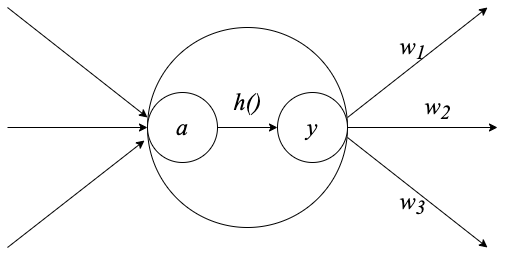
\includegraphics[width=8cm]{images/Hidden_Layer_Node.png}
    \caption{Inside Structure of a node in the Hidden Layer. The output value from the previous layer is stored as value $a$ and then modified to value $y$ by the activation function $h()$. $y$ becomes the output for this node and will be passed down to the next layer with the multiplication of their respective weight parameter $\textbf{w}$}
    \label{fig:hidden_layer}
\end{figure}

Activation function $h$ acts as a decision point whether the inputted data should be passed on to the next neuron or not. This paper would introduce one of the fundamental and commonly used activation function called the Sigmoid Function (equation (\ref{eq:Sigmoid}), Figure \ref{fig:Sigmoid}) and the more recently developed activation function called Leaky Rectified Linear Unit (Leaky ReLU) (equation (\ref{eq:LeakyReLU}), Figure \ref{fig:LeakyReLU}) made by \citet{LeakyReLU}.

Assuming an input data $x$, the Sigmoid function (\ref{eq:Sigmoid}) and the Leaky ReLU are defined as:

\begin{align}
    h(x)& = \frac{1}{1+e^{-x}}\label{eq:Sigmoid}, \\
    h(x)& = \left\{\begin{array}{ll}
    x & (\text { if } x \geq 0) \\
    \frac{x}{a} & (\text { if } x<0),
    \end{array}\right\label{eq:LeakyReLU}
\end{align}
where $a$ is a fixed parameter in the range $(1, +\infty)$. According to \citet{LeakyReLU}, $a$ is preferred to be a large number such as $a = 100$. However, in an empirical study done by \citet{LeakyReLu_a}, they concluded that $a = 5.5$ performed well than other numbers. Therefore, this paper will adopt $a=5.5$ for our leaky ReLU parameter. 

\begin{figure}[!ht]
    \centering
    \begin{minipage}{.5\textwidth}
        \centering
        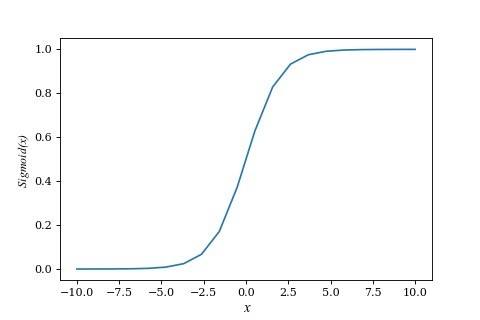
\includegraphics[width=7cm]{images/Sigmoid.png}
        \captionof{figure}{A line plot of a Sigmoid \\function.}
        \label{fig:Sigmoid}
    \end{minipage}%
    \begin{minipage}{.5\textwidth}
        \centering
        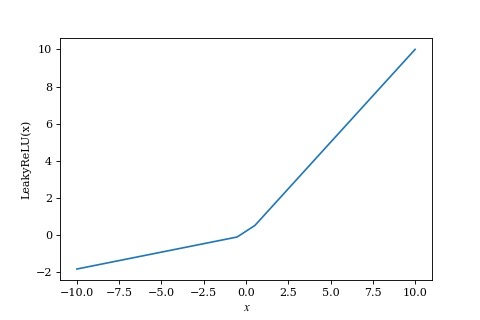
\includegraphics[width=7cm]{images/LeakyReLU.png}
        \captionof{figure}{A line plot of a Leaky ReLU function. }
        \label{fig:LeakyReLU}
    \end{minipage}%
\end{figure}

The activation function in the output layer is different with the function used in the hidden layer. In a regression problem, there should be one final output which reflects all of the information from the outputted data of the previous layer, and to do so we use the Identity Function $I$ defined as:
\begin{equation}
    I(x) = x.
\end{equation}

The biggest advantage of using a neural network is that the network is able to optimize its parameters using training data and accurately adapt to the features of the input data. By setting the loss function $E$ and getting the gradient of this loss function $E$, we get the indication if the neural network is accurately reflecting the features of the inputted data. For a regression problem we set Sum of Squared Error (SSE) as the loss function which is defined as:
\begin{equation}\label{eq:SSE}
    \mathrm{E} = \mathrm{SSE} = \frac{1}{2} \sum_{i=1}^{N}\left(y_{i}-t_{i}\right)^{2},
\end{equation}
where $N$ is the amount of input data, $y$ as the outputted value from the neural network, and $t$ as the correct data which corresponds to the $i$th value in the outputted data. Using the loss function $E$ we optimize the weight and bias parameters by the calculation:
\begin{align}
    \hat{w_{i j}} &= w_{i j} - \eta \frac{\partial E}{\partial w_{i j}},\label{eq:trainW}\\
    \hat{b_{i j}} &= b_{i j} - \eta \frac{\partial E}{\partial b_{i j}}\label{eq:trainb},
\end{align}
where $\hat{w_{i j}}, \hat{b_{i j}}$ is the updated parameter value of the weight and bias, and $\eta$ is the learning rate. This modification is aimed to decrease the gradient of the loss function and when the gradient becomes close to 0, we can conclude that the training of neural network is finished. Generally when calculating the gradient of the loss function we use a calculation algorithm called Backpropagation which calculates the error term from the output layer to the previous iteration using the chain rule. Using this algorithm, it is possible to achieve a faster and more efficient way to calculate the gradient. 

Another essential concept within DNN is the optimizer. The optimization method shown shown in equations (\ref{eq:trainW})(\ref{eq:trainb}), is called the Stochastic Gradient Descent (SGD), which calculates the gradient from a randomly chosen data. This optimizer however, entails some detrimental issue where the convergence of the gradient is hard to achieve because of the amount of noise the approximation process consist. When the gains are decreasing too slowly, the variance of parameter estimate decreases equally slow. If the gains decrease too quickly on the other hand, the parameter estimate takes a very long time to approach its optimum \citep{SGD_problem}. Although SGD is a well-known practice with promising results other methods which curves the underlying issue of this method are developed. 

One of the promising alternative optimizer is the Adaptive Moment Estimation (Adam) \citep{Adam} which integrated the features of two optimizers; Momentum \citep{Momentum} and Adaptive Gradient Algorithm (Adagrad) \citep{Adagrad}. Below would demonstrate the fundamental theory of Adam referring from the works of \citet{optimizers}. This algorithm consists of two components; the component of gradient by setting the exponential moving average of past gradients $m$, and the component of learning rate by setting the exponential moving average of past squared gradients $v$. We compute the two moving averages by:

\begin{align}
    m_{t} &=\beta_{1} m_{t-1}+\left(1-\beta_{1}\right) g_{t} \\
    v_{t} &=\beta_{2} v_{t-1}+\left(1-\beta_{2}\right) g_{t}^{2}
\end{align}
where $m_{t}$ and $v_{t}$ are estimates of the first moment, and the second moment of the gradients respectively. $m_{t}$ and $v_{t}$ are initialized in vector 0s and \citet{Adam} argues that these estimates are biased towards 0. To account for the biases existing in the vectors, Adam optimizer sets the bias correction as:

\begin{align}
    \hat{m}_{t} &=\frac{m_{t}}{1-\beta_{1}^{t}},\\
    \hat{v}_{t} &=\frac{v_{t}}{1-\beta_{2}^{t}}.
\end{align}
This will yield the Adam optimizer defined as:
\begin{equation}
    \theta_{t+1}=\theta_{t}-\frac{\eta}{\sqrt{\hat{v}_{t}}+\epsilon} \hat{m}_{t},
\end{equation}
where $\eta$ is the learning rate and $\theta$ is the parameter in which we are optimizing. Figures \ref{fig:SGD} and \ref{fig:Adam} shows the path of each optimizers. We could indicate that the SDG oscillates between the field of gradient and thus have a redundant path over Adam. Note that this does not however undermine the effectiveness of SGD, but merely stating that SGD takes more iterations to get to the optimum. 

There are many other optimization algorithms existing in the field of neural networks. However, this paper will primarily be using Adam for the optimizer hence, will not cover any other optimizers. 

\begin{figure}[!ht]
    \centering
    \begin{minipage}{.5\textwidth}
        \centering
        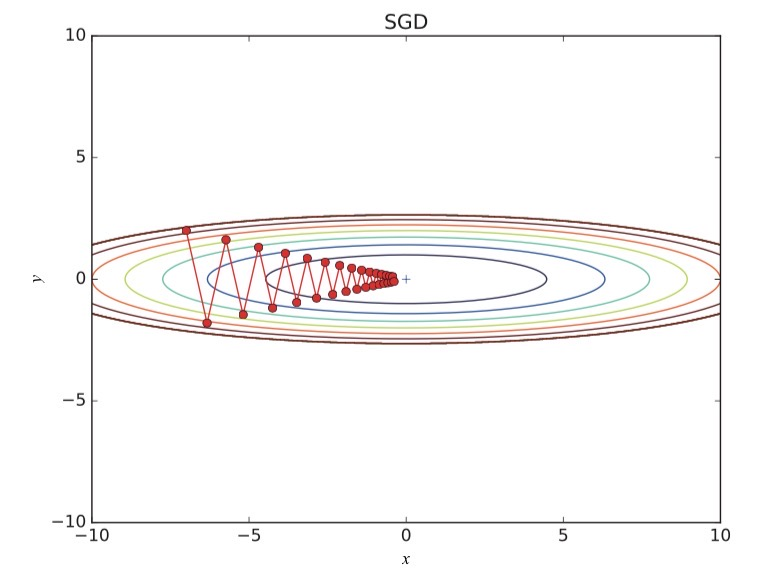
\includegraphics[width=7.5cm]{images/SGD.png}
        \captionof{figure}{The path of SGD optimizer \\We can see that it has an inefficient rou-\\te to the optimum. \citep{DLfromscratch}}
        \label{fig:SGD}
    \end{minipage}%
    \begin{minipage}{.5\textwidth}
        \centering
        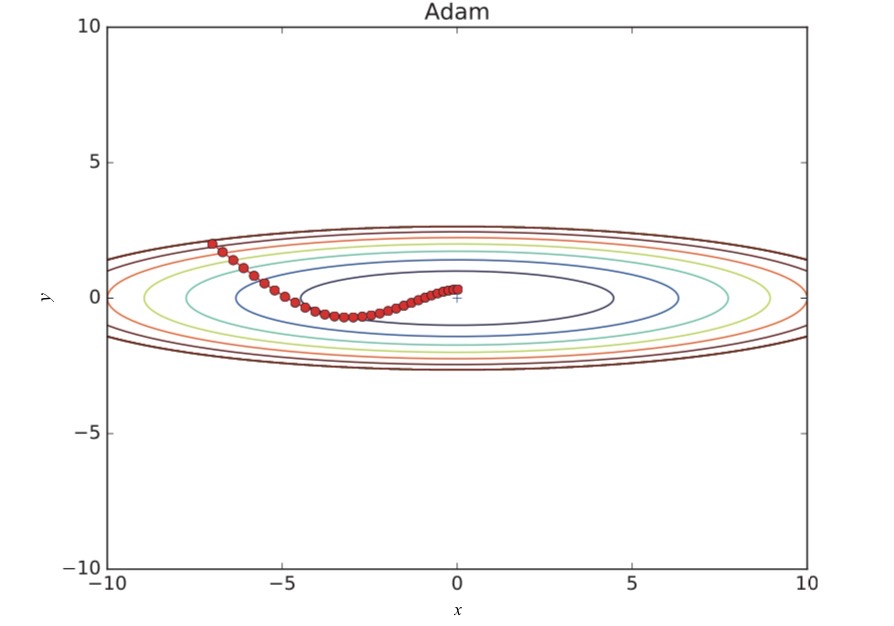
\includegraphics[width=7.5cm]{images/Adam.png}
        \captionof{figure}{The path of Adam optimizer \\The path efficiently goes to the optimum\\ \citep{DLfromscratch}}
        \label{fig:Adam}
    \end{minipage}%
\end{figure}

This was the basic construct of a neural network used in a regression problem. In a classification problem, despite the structure of the network being the same, the activation function and the loss function used is different. However, this paper will omit the explanation of a classification problem since it is out of the research scope of this paper. 

\subsubsection{RNN Model}
Recurrent Neural Network (RNN) is a type of neural network which is widely used pertaining to research and studies in time series data. The key component of RNNs is that it can store information about the pattern of sequence. Using the output of the previous iteration of the RNN layer as the input for the next layer, the network is able to recognize the features of a sequence of time series data. 
\begin{figure}[ht]
    \centering
    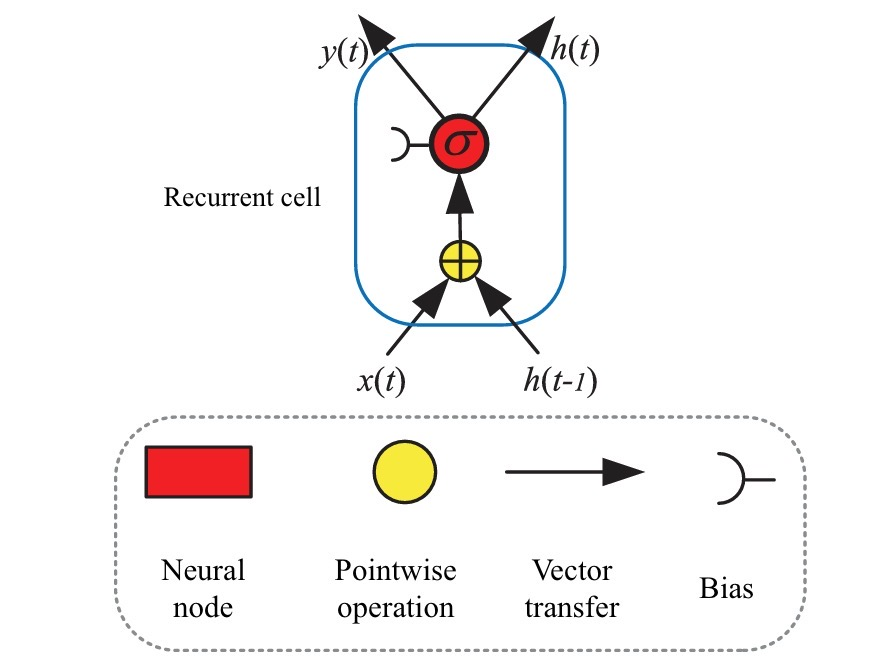
\includegraphics[width=9cm]{images/RNN.png}
    \caption{The Structure of a RNN node \citep{LSTM_GRU_description}. We could see that the node consists of multiple operations and has two inputs, which are, an input of the given timestamp, and an input from the hidden layer of the previous iteration.}
    \label{fig:RNN}
\end{figure}

Figure \ref{fig:RNN} shows the basic structure of standard recurrent sigma cell. The fundamental difference with a normal DNN is that RNN has a recurrent cell in the hidden unit. The recurrent cell takes the state of the previous iteration as the input which achieves the passing of previous sequential information. Let us assume that in time $t$ we denote $x_{t}$ as the input data, $h_{t}$ as the recurrent information, and $y_{t}$ as the output data. We can define the output data as:

\begin{align}
    h_{t} &= \sigma\left(W_{h} h_{t-1}+W_{x} x_{t}+b\right), \\
    y_{t} &= h_{t},
\end{align}

\noindent where $b$ is the bias, $W_{h}$ and $W_{x}$ are the weight of hidden-to-hidden connection, and input-to-hidden connection respectively. $\sigma$ is the activation function within the hidden layer. The method of optimizing parameters does not differ significantly with DNN. However, the way we compute the gradient of the loss function $E$ differs with DNN since it requires us to expand the computation steps to go back one step at a time to obtain the dependencies among multiple variables and parameters of RNN. Therefore, replacing the normal Backpropagation algorithm utilized in DNNs, we apply Backpropagation Through Time (BPTT) algorithm to calculate the gradients. In this paper however, it would not go over the specific calculation of BPTT since it is out of the scope of this paper.

\subsubsection{LSTM Model}
RNN performs very strongly in a wide domain of research questions such as speech recognition, natural language processing and various prediction questions in Economics. However, from the research done by \citet{RNN_problem} training RNN presented issues of gradient vanishing and exploding problem, which both causes detrimental effect in the training process of parameters. Furthermore, a more recent research by \citet{RNN_longtermdependency_issue} have found that the RNN is incapable of adequately handling information of the past when the gap of the relevant time series data becomes wide. Addressing these issues, Long Short-Term Memory (LSTM) model was developed by \citet{LSTM} which added the concept of "\textbf{gates}" into standard RNN to increase the capacity of its memory. Succeeding the works of \citet{LSTM}, \citet{LSTM_forget_gate} modified the LSTM structure by adding a \textit{forget gate} which became the new standard of LSTM. 

\begin{figure}[ht]
    \centering
    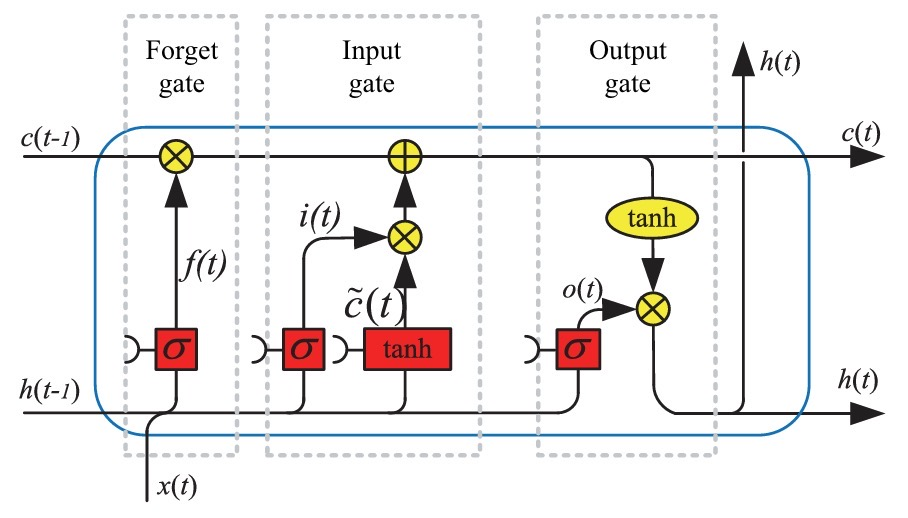
\includegraphics[width=12cm]{images/LSTM.png}
    \caption{The Structure of LSTM node \citep{LSTM_GRU_description}. The structure is identical with the RNN node but its complexity has increased. The gates within the node is each designed to interpret long sequences which RNN was unable to achieve.}
    \label{fig:LSTM}
\end{figure}

Figure \ref{fig:LSTM} shows the overview of the LSTM cell block. We see that there are several gates inside the cell which are indicated as \textit{Forget gate}, \textit{Input gate}, and \textit{Output gate}. Let us denote $c_{t}$, $f_{t}$, $i_{t}$, $o_{t}$ as the cell state, forget gate, input gate, and output gate of LSTM at time $t$ respectively and $x_{t}$ as the input data. The mathematical expression of Figure \ref{fig:LSTM} can be expressed as:
\begin{align}
    f_{t} &= \sigma(W_{fh}h_{t-1} + W_{fx}x_{t} + b_{f}),\label{eq:LSTM1}\\
    i_{t} &= \sigma(W_{ih}h_{t-1} + W_{ix}x_{t} + b_{i}),\label{eq:LSTM2}\\
    \tilde{c}_{t} &= \mathrm{tanh}(W_{\tilde{c}_h}h_{t-1} + W_{\tilde{c}x}x_{t} + b_{\tilde{c}}),\label{eq:LSTM3}\\
    c_{t} &= f_{t}\cdot c_{t-1} + i_{t} \cdot \tilde{c}_{t},\label{eq:LSTM4}\\
    o_{t} &= \sigma(W_{oh}h_{t-1} + W_{ox}x_{t} + b_{o}),\label{eq:LSTM5}\\
    h_{t} &= o_{t} \cdot \mathrm{tanh}(c_{t}),\label{eq:LSTM6}
\end{align}
where $W_{\alpha \beta}$ is the weight of the $\alpha$-to-$\beta$  connection (e.g. $W_{f x}$ is the weight value of forget gate-to-input data connection), $b$ is the bias term corresponding to the gates, $\tilde{c}_{t}$ represents the candidate of cell state of the given time stamp which will be used in the computation of cell state $c_{t}$ in the output gate (shown in equation (\ref{eq:LSTM3})), $h_{t}$ is the output of this LSTM cell block, $\sigma$ is the activation function, and the operator ‘·’ denotes the pointwise multiplication of two vectors. 

The input gate decides the new information stored in the cell state, the forget gate determines how much information from the previous iteration would be passed on to the current cell with values ranging from 1 (passes on all data) to 0 (omits all data from previous cell), and finally the output gate decides what information can be outputted based on the cell state.  

\subsubsection{GRU Model}
Utilizing this LSTM structure, we became capable of handling the long-term dependencies and remedy the issues pertaining to the computation of gradients presented in the standard RNN. However, the addition of parameters attributed to the concept of gates intensified the computational complexity. To modify, as well as simplify the LSTM structure, \citet{GRU} developed the Gradient Recurrent Unit (GRU) Model which consisted of only two gates; the Reset gate and the Update gate. 

\begin{figure}[ht]
    \centering
    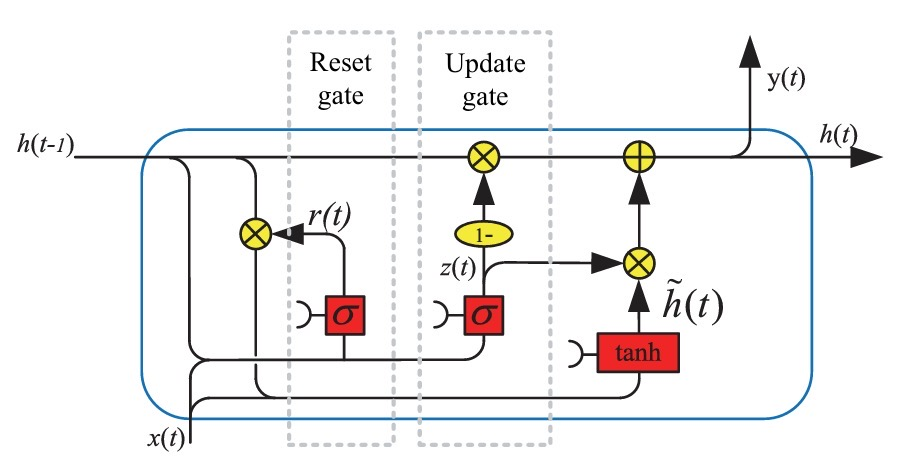
\includegraphics[width=12cm]{images/GRU.png}
    \caption{The Structure of GRU node \citep{LSTM_GRU_description}. The structure has decreased its complexity compared to LSTM only having two gates. This accounts for the decrease of parameters used which significantly affects the speed of training.}
    \label{fig:GRU}
\end{figure}

Figure \ref{fig:GRU} shows the basic construct of the GRU. Compared with Figure \ref{fig:LSTM}, we can see that the overall cell structure does not have a drastic change but the amount of notations and gates inside the cell have decreased. Let us denote $r_{t}$ and $z_{t}$ as the reset gate and the update gate respectively. The mathematical expression of Figure \ref{fig:GRU} can be expressed as: 
\begin{align}
    r_{t} &=\sigma\left(W_{r h} h_{t-1}+W_{r x} x_{t}+b_{r}\right), \\ z_{t} &=\sigma\left(W_{z h} h_{t-1}+W_{z x} x_{t}+b_{z}\right), \\ \tilde{h}_{t} &=\mathrm{tanh} \left(W_{\tilde{h} h}\left(r_{t} \cdot h_{t-1}\right)+W_{\tilde{h} x} x_{t}+b_{z}\right), \label{eq:GRU_output}\\ 
    h_{t} &=\left(1-z_{t}\right) \cdot h_{t-1}+z_{t}, \cdot \tilde{h}_{t},
\end{align}
where $W$ and $b$ are the weight and bias parameters respectively which corresponds with each gates, $\sigma$ is the activation function, and $\tilde{h}_{t}$ represents the candidate of output of the given time stamp which will be integrated in the computation of output $h_{t}$ of this GRU cell block which is shown in equation (\ref{eq:GRU_output}).

Using less parameters than LSTM, GRU is capable of training its parameters in a rapid nature. However, some studies such as \citet{LSTM_GRU_comparison} have concluded that when the complexity of the input increases, LSTM performed better than GRU. 

In this paper, we aim to use these methodologies to compare the results between conventional methods as well as advanced deep learning methods to determine the best performing method for predicting COVID-19 positive rates. For the formulation of prediction models we use the Keras library provided by \citet{keras}.